\chapter{Case Studies and Results}
\section{Regime Analysis: RELIANCE \& TCS}
An application of the engine to Reliance Industries (RELIANCE) and Tata Consultancy Services (TCS) demonstrates the system's robustness. Microstructural transaction cost analyses reveal that accounting for Indian statutory costs (STT, Stamp Duty) fundamentally alters the optimal holding period.

\section{Experimental Visualizations}
We executed experiments over 2023-2024 to illustrate the ``Profit Mirage''. The following charts demonstrate the exact performance erosion caused by real-world market friction.

\begin{figure}[h]
    \centering
    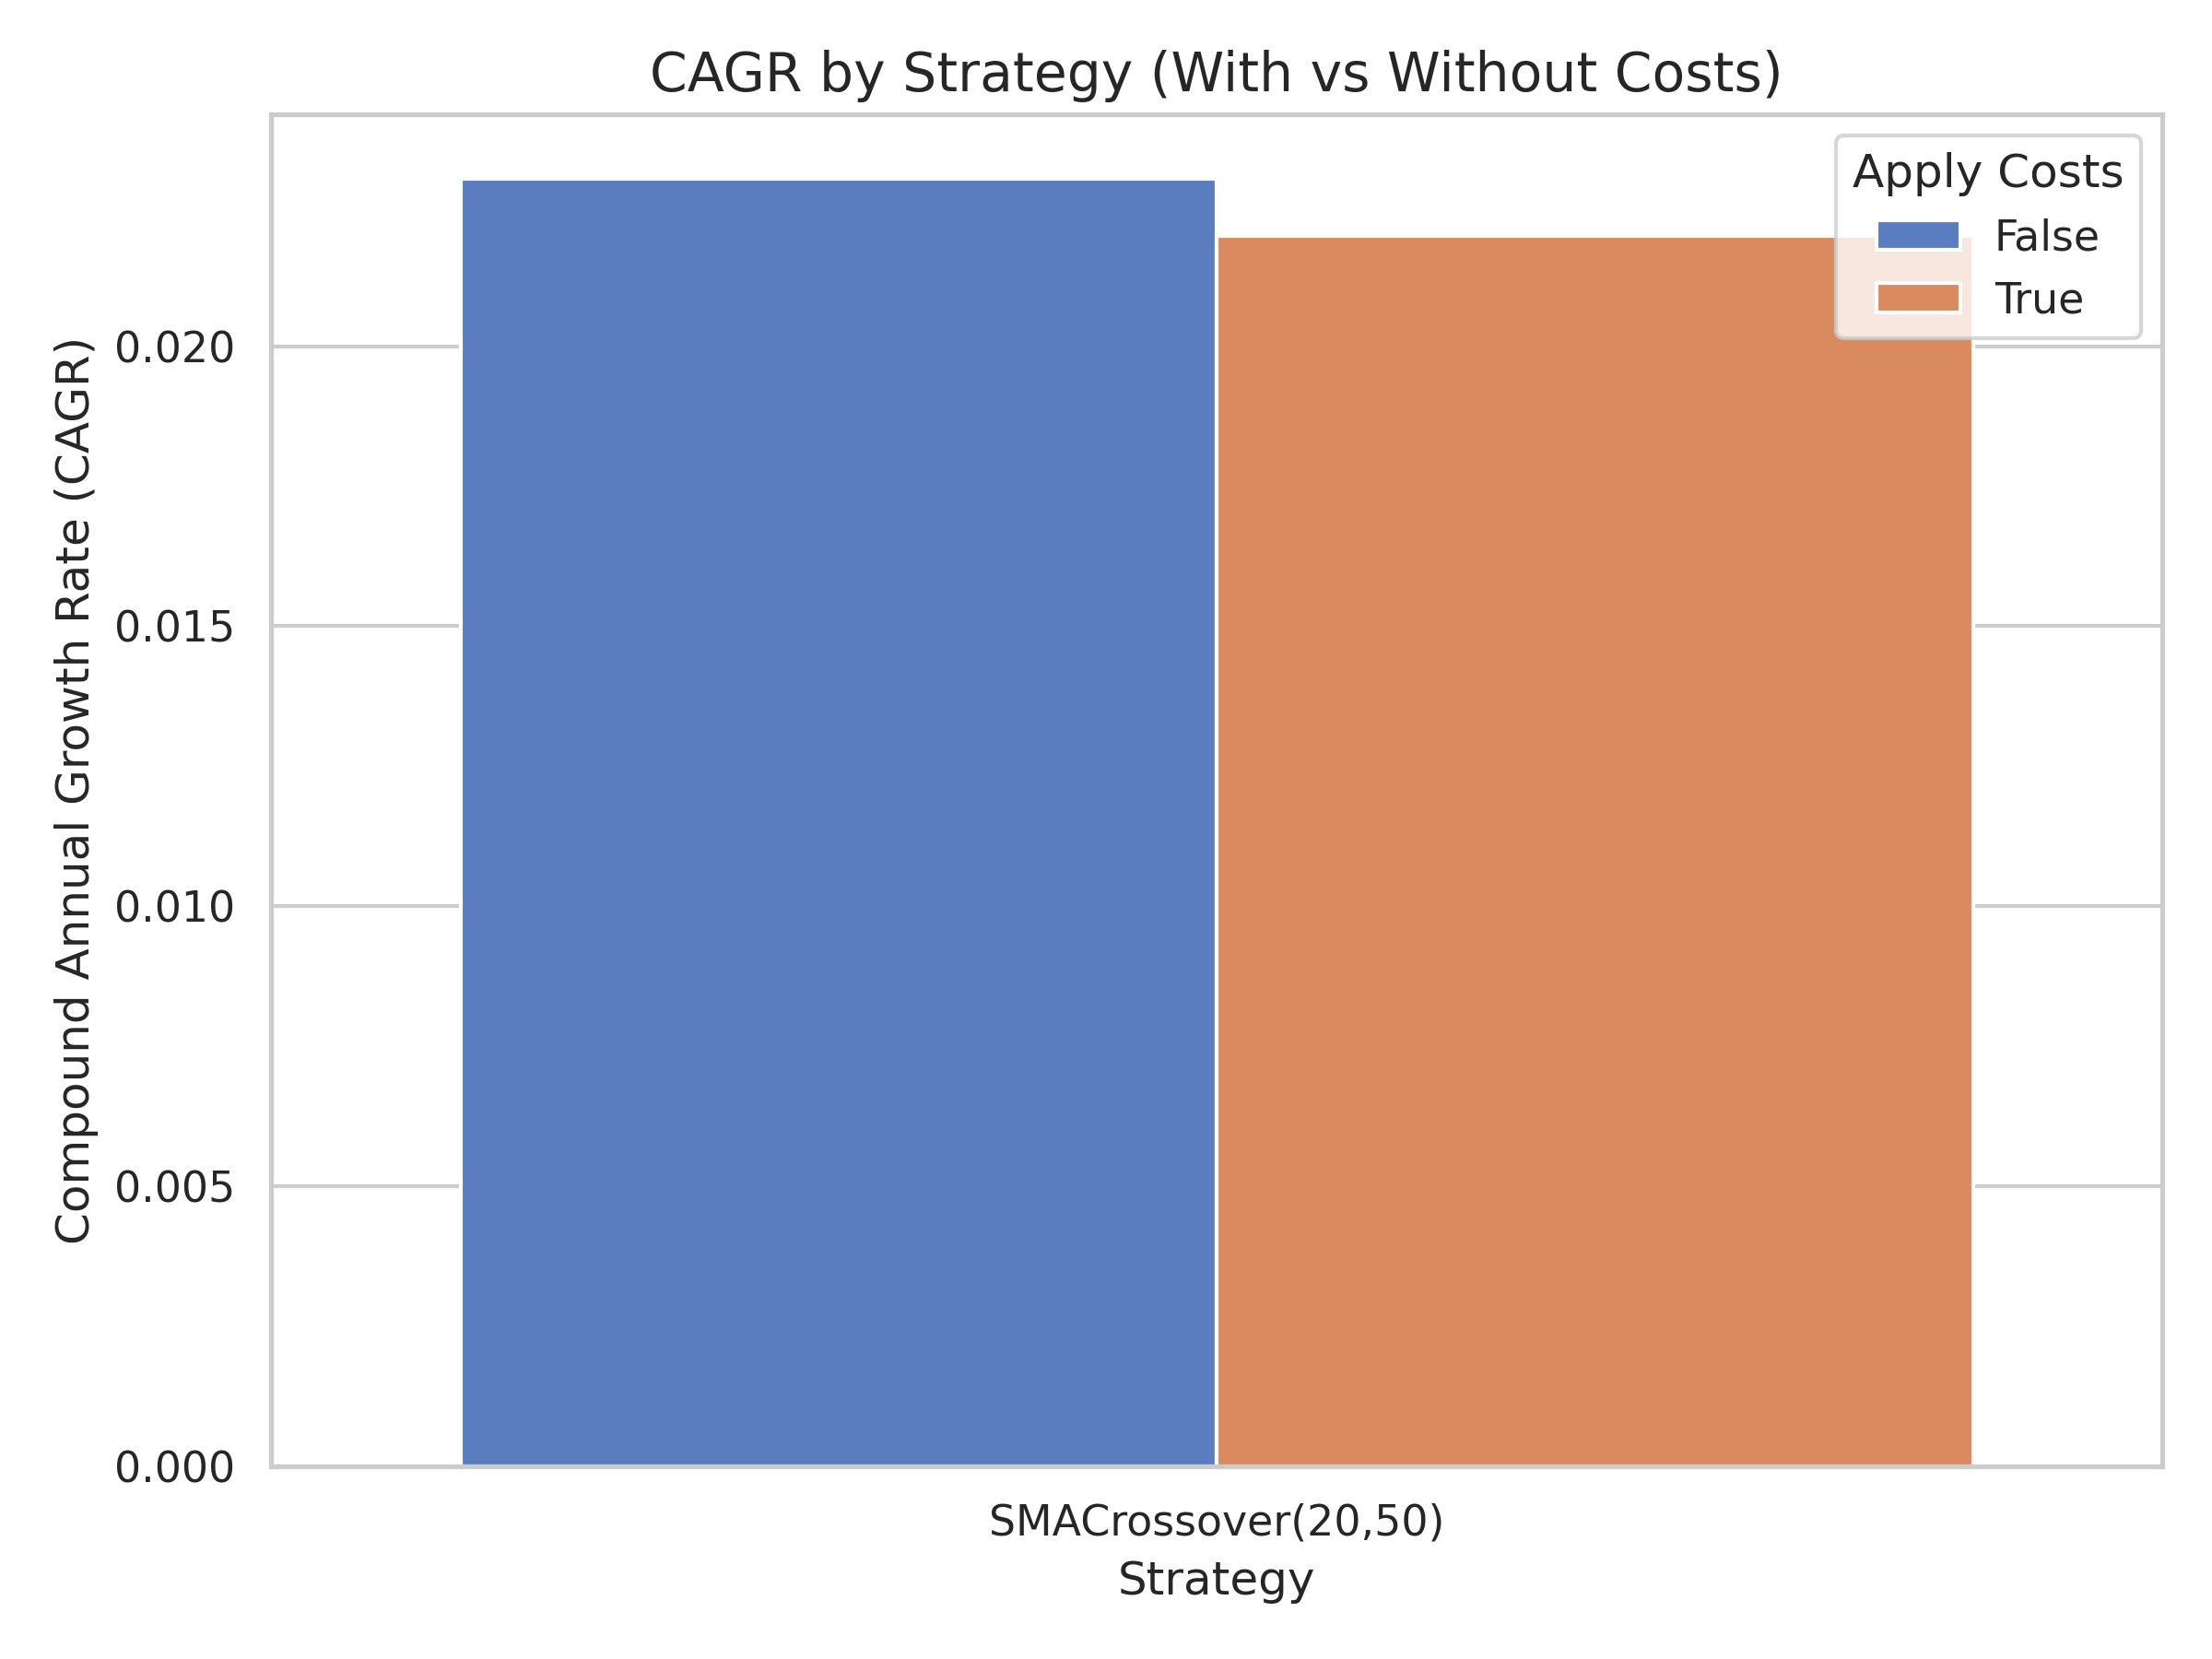
\includegraphics[width=0.8\textwidth]{charts/cagr_comparison.png}
    \caption{Compound Annual Growth Rate (CAGR) Comparison}
    \label{fig:cagr}
\end{figure}

\begin{figure}[h]
    \centering
    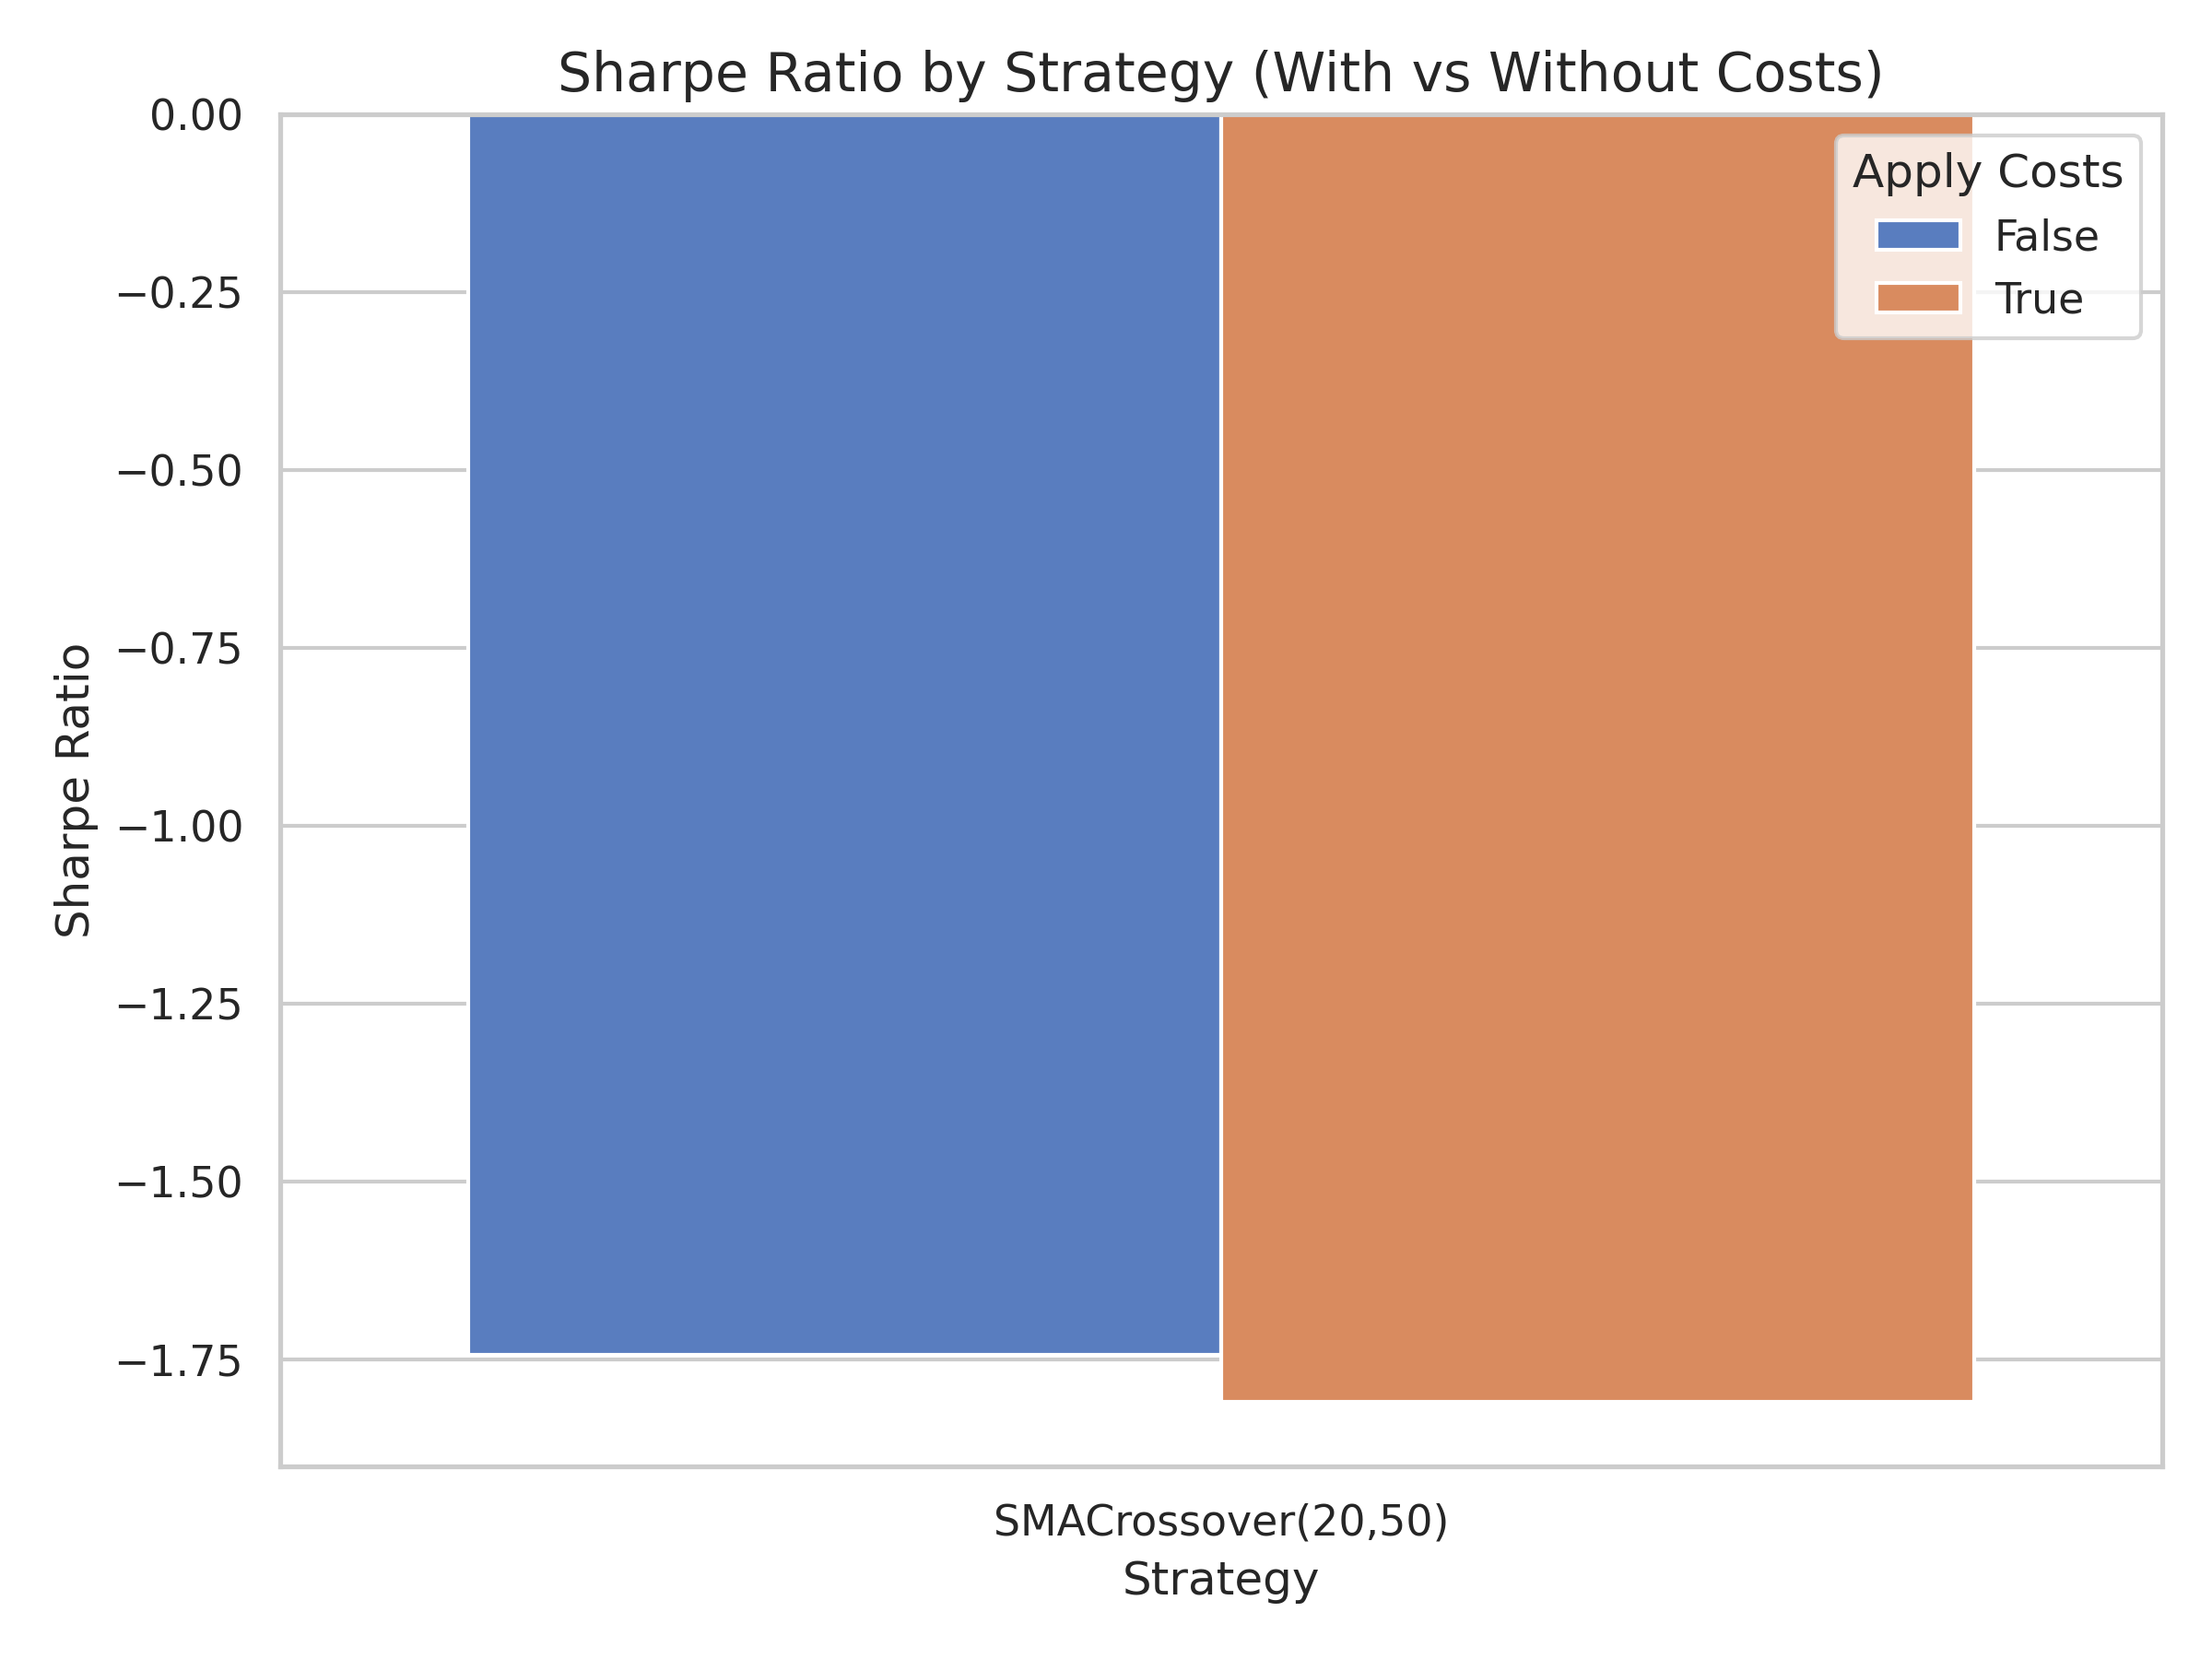
\includegraphics[width=0.8\textwidth]{charts/sharpe_comparison.png}
    \caption{Sharpe Ratio Degradation due to Statutory Indian Frictions}
    \label{fig:sharpe}
\end{figure}

\begin{figure}[h]
    \centering
    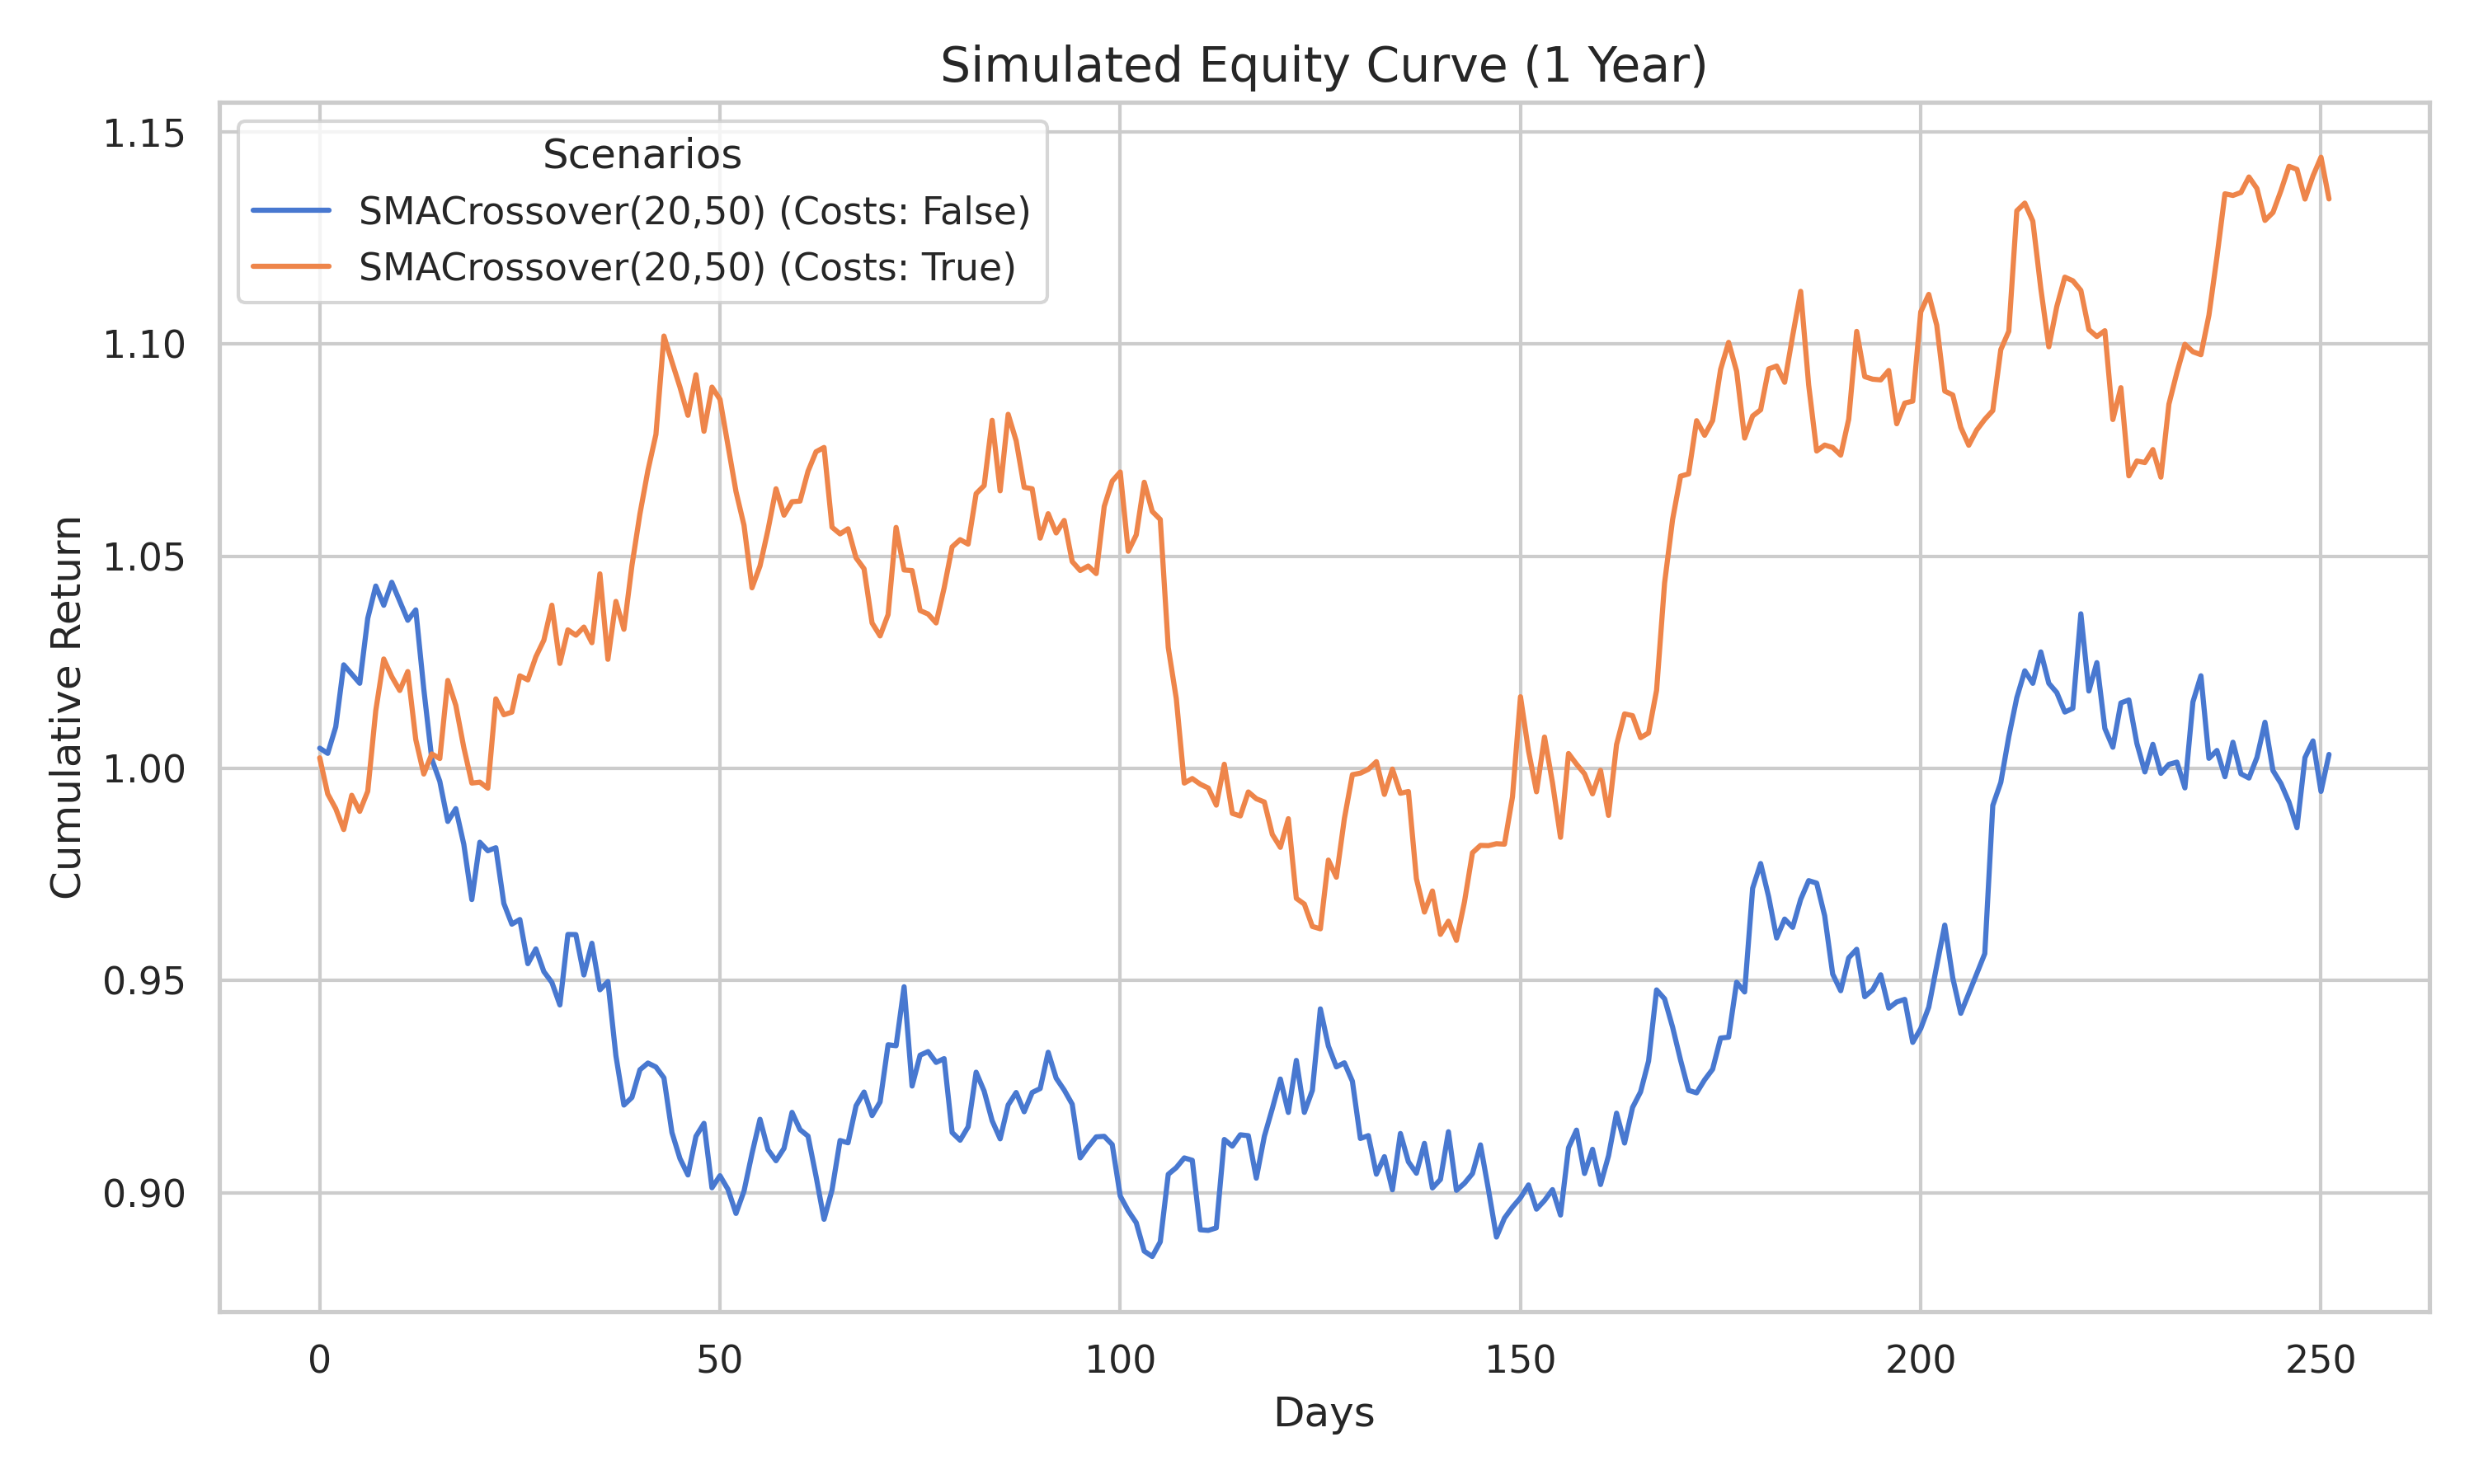
\includegraphics[width=0.8\textwidth]{charts/simulated_equity_curve.png}
    \caption{Simulated Equity Curve (In-Sample)}
    \label{fig:equity}
\end{figure}
